\section{Matrícula mercantil (RUES)}

El segundo capítulo examina la huella mercantil del egresado. Al cruzar las cédulas de los cerca de 174.685 graduados de las seis sedes con el Registro Único Empresarial y Social, \num{37544} de ellos ---alrededor del 21,5\,\% del total--- aparecen como titulares de una matrícula mercantil. Como en el capítulo anterior, la pregunta deja de ser cuántos se registran en el RUES para volverse qué tipo de empresa crean, en qué sector, con qué supervivencia y desde qué carrera y territorio. Conviene advertir desde el principio una restricción que condiciona todo el capítulo: el enlace por cédula solo recupera a quien figura como persona natural comerciante, no a quien se registra en el RUES a través de una sociedad identificada por NIT, de modo que las cifras que siguen describen la matrícula mercantil individual y no la actividad societaria.

\subsection{Naturaleza jurídica de las empresas}
La Tabla~\ref{tab:rues_org} hace explícita esa restricción. La práctica totalidad de las matrículas enlazadas ---el 99,9\,\%--- corresponde a persona natural, sencillamente porque las sociedades se identifican con NIT y no con la cédula de sus socios, de modo que el cruce no las alcanza. La matrícula mercantil que este capítulo describe es, por tanto, la del egresado que registra negocio a su propio nombre ---el comerciante individual, el profesional independiente formalizado---, y no el de quien constituye una compañía. Se trata de un límite estructural más que de un hallazgo: el NIT queda fuera del alcance del enlace, así que la medición subestima la matrícula mercantil real. Cuanto sigue debe leerse con esa salvedad, que se retoma al cierre como límite principal.

\begin{table}[H]\centering\footnotesize
\caption{Matrículas de los graduados por \textbf{organización jurídica} (RUES).}\label{tab:rues_org}
\begin{tabular}{lr}
\toprule
\rowcolor{ustaazul}\textbf{\color{white}Organización jurídica} & \textbf{\color{white}\% de matrículas} \\
\midrule
Persona Natural & 99,9\% \\
Sociedad Limitada & 0,0\% \\
Otras Sociedades & 0,0\% \\
Empresas Asociativas De Trabajo & 0,0\% \\
Empresas Unipersonales & 0,0\% \\
\bottomrule
\end{tabular}
\\[2pt]{\scriptsize\color{ustagris} El cruce por cédula capta sobre todo persona natural; las sociedades con NIT no se enlazan por la cédula del socio.}
\end{table}

\subsection{Sector económico de las empresas}
Clasificando la actividad principal de cada matrícula por su código CIIU (Tabla~\ref{tab:rues_sector} y Figura~\ref{fig:ruessector}), el perfil sectorial del matriculado en el RUES tomasino es inequívoco. El comercio encabeza con holgura, con 9.535 matriculados en el RUES y el 25,4\,\% del total, seguido del alojamiento y la comida ---restaurantes, cafeterías, hospedaje--- con 3.841 matriculados en el RUES y el 10,2\,\%, y de las actividades profesionales y técnicas con 3.499 y el 9,3\,\%. Más atrás aparecen la industria manufacturera (5,0\,\%), la salud y la asistencia social (3,9\,\%), los servicios administrativos (3,3\,\%) y la construcción (2,9\,\%). El retrato es el de una matrícula mercantil de proximidad: comercio al por menor y servicios de consumo cotidiano, antes que actividades intensivas en capital o conocimiento.

\begin{table}[H]\centering\footnotesize
\caption{Sector económico de las empresas de los graduados, según \textbf{CIIU} (RUES).}\label{tab:rues_sector}
\begin{tabular}{lrr}
\toprule
\rowcolor{ustaazul}\textbf{\color{white}Sector económico (CIIU)} & \textbf{\color{white}Matriculados} & \textbf{\color{white}\%} \\
\midrule
Comercio & 9.535 & 25,4\% \\
Alojamiento y comida & 3.841 & 10,2\% \\
Profesionales y técnicas & 3.499 & 9,3\% \\
Industria manufacturera & 1.869 & 5,0\% \\
Salud y asistencia social & 1.454 & 3,9\% \\
Servicios administrativos & 1.251 & 3,3\% \\
Construcción & 1.077 & 2,9\% \\
Transporte y logística & 832 & 2,2\% \\
Educación & 796 & 2,1\% \\
Otros servicios & 789 & 2,1\% \\
\bottomrule
\end{tabular}
\\[2pt]{\scriptsize\color{ustagris} Sector de la actividad principal (división CIIU de la matrícula representativa de cada cédula).}
\end{table}

\begin{figure}[H]\centering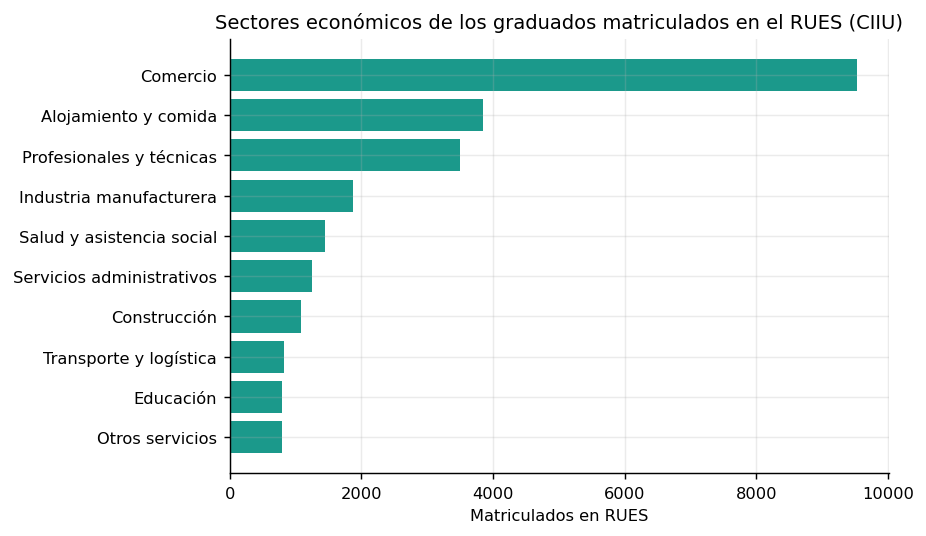
\includegraphics[width=0.74\linewidth]{figs_cruce/R1_rues_sector.png}
\caption{Sectores económicos (CIIU) de las empresas registradas por los graduados.}\label{fig:ruessector}\end{figure}

\subsection{Matrícula mercantil por carrera}
La Tabla~\ref{tab:rues_carrera} ordena los programas por número de graduados con matrícula mercantil. El Derecho vuelve a encabezar, con \num{3393} matriculados en el RUES, seguido de la Contaduría Pública (\num{2328}), la Economía (\num{1914}), los Negocios Internacionales (\num{1903}) y la Arquitectura (\num{1879}). La jerarquía reproduce en buena medida el tamaño de cada programa, pero la columna de empresa activa introduce un primer matiz: los Negocios Internacionales (44,7\,\%) y la Administración de Empresas (41,7\,\%) destacan muy por encima del promedio, mientras que programas como la Economía (24,7\,\%) o la Licenciatura en Educación Preescolar (16,3\,\%) se quedan por debajo. Como se verá, buena parte de ese contraste responde a la antigüedad de las matrículas y no a una solidez intrínseca del programa.

\begin{table}[H]\centering\footnotesize
\caption{Matrícula mercantil por \textbf{carrera}: programas con más graduados matriculados en el RUES.}\label{tab:rues_carrera}
\begin{tabular}{lrrr}
\toprule
\rowcolor{ustaazul}\textbf{\color{white}Programa (carrera)} & \textbf{\color{white}Matriculados} & \textbf{\color{white}Matrículas} & \textbf{\color{white}\% activa} \\
\midrule
Derecho & 3.393 & 3.951 & 29,0\% \\
Contaduria Publica & 2.328 & 2.809 & 27,0\% \\
Economia & 1.914 & 2.408 & 24,7\% \\
Negocios Internacionales & 1.903 & 2.275 & 44,7\% \\
Arquitectura & 1.879 & 2.392 & 30,8\% \\
Ingenieria Civil & 1.629 & 2.010 & 32,4\% \\
Especializacion En Derecho Adm & 1.248 & 1.493 & 21,4\% \\
Odontologia & 1.234 & 1.521 & 35,7\% \\
Administracion De Empresas & 1.180 & 1.372 & 41,7\% \\
Psicologia & 855 & 977 & 26,8\% \\
Administracion De Empresas Agr & 751 & 942 & 44,1\% \\
Licenciatura En Educacion Pree & 750 & 905 & 16,3\% \\
\bottomrule
\end{tabular}
\\[2pt]{\scriptsize\color{ustagris} Programa principal de cada graduado matriculado. Ordenado por nº de matriculados.}
\end{table}

\subsection{Sector económico por carrera}
Aquí surge el contraste más interesante con el capítulo de contratación pública. En el SECOP, cada profesión contrataba en su especialidad; en el RUES, la Figura~\ref{fig:ruescarrerasector} muestra que casi todas las carreras se registran en el RUES, ante todo, en el comercio: el egresado que crea empresa suele abrir un negocio, no ejercer su profesión por cuenta propia. El Derecho (42,4\,\% comercio), la Contaduría (48,7\,\%), la Economía (48,0\,\%) y los Negocios Internacionales (53,0\,\%) confirman ese patrón. Solo unas pocas disciplinas trasladan su formación al objeto de su empresa: la Odontología se registra en el RUES en salud (57,8\,\%), la Arquitectura en servicios profesionales y técnicos (36,0\,\%) y la Ingeniería Civil reparte su actividad entre el comercio (26,8\,\%) y la construcción (31,0\,\%). El título, que en la contratación pública determinaba el objeto del contrato, en la matrícula mercantil se diluye: salvo en la salud y en algunos servicios técnicos, el graduado se registra en el RUES como comerciante antes que como profesional de su disciplina.

\begin{figure}[H]\centering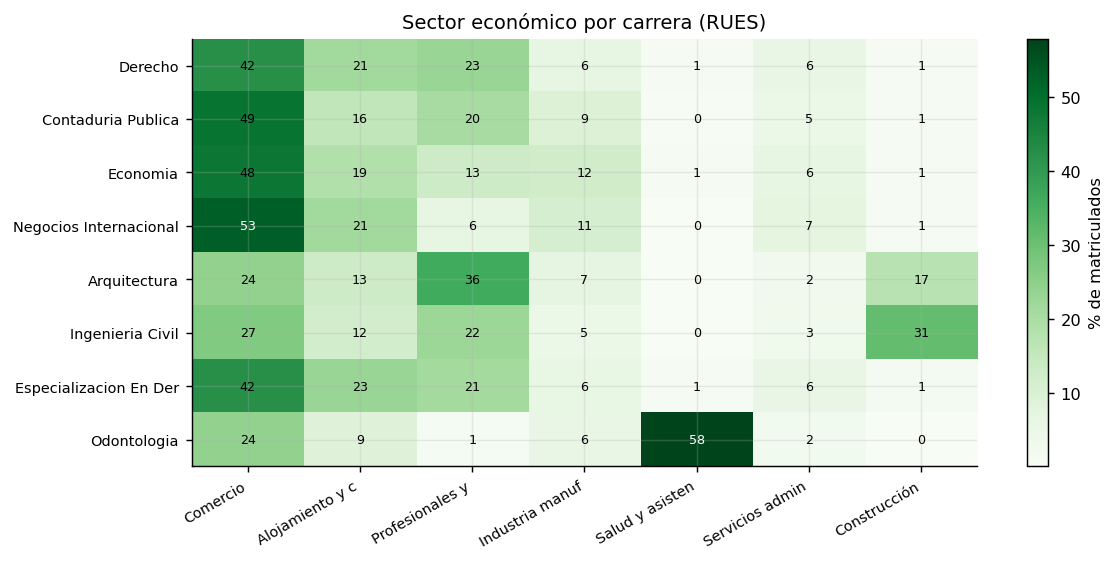
\includegraphics[width=0.94\linewidth]{figs_cruce/R2_rues_carrera_sector.png}
\caption{Sector económico de la empresa por carrera (\% de matriculados en el RUES por fila). El comercio domina en casi todos los programas; la salud y los servicios técnicos son las excepciones disciplinares.}\label{fig:ruescarrerasector}\end{figure}

\subsection{Supervivencia empresarial}
De las matrículas enlazadas, el 73,4\,\% figura como cancelada y solo el 24,7\,\% sigue activa (Tabla~\ref{tab:rues_estado}); contando por persona ---activa si conserva al menos una empresa viva---, \num{11125} matriculados en el RUES, el 29,6\,\%, mantienen actividad. Esa supervivencia no se reparte por igual entre carreras: como muestra la Figura~\ref{fig:ruessupcarrera}, programas como la Optometría (59,2\,\%), la Ingeniería Ambiental (56,0\,\%) o la Ingeniería Industrial (53,1\,\%) presentan las tasas de empresa activa más altas, frente a otros que apenas superan el 39\,\%.

\begin{table}[H]\centering\footnotesize
\caption{Estado de las matrículas de los graduados (RUES).}\label{tab:rues_estado}
\begin{tabular}{lr}
\toprule
\rowcolor{ustaazul}\textbf{\color{white}Estado de la matrícula} & \textbf{\color{white}\% de matrículas} \\
\midrule
Cancelada & 73,4\% \\
Activa & 24,7\% \\
Matrícula Cancelada Por Traslado De Domicilio & 0,8\% \\
Matrícula Cancelada Ley 1429 & 0,8\% \\
Matrícula Nueva, Constitución Por Traslado & 0,1\% \\
Matricula Inactiva Por Perdida De Calidad De Comerciante & 0,1\% \\
\bottomrule
\end{tabular}
\end{table}

\begin{figure}[H]\centering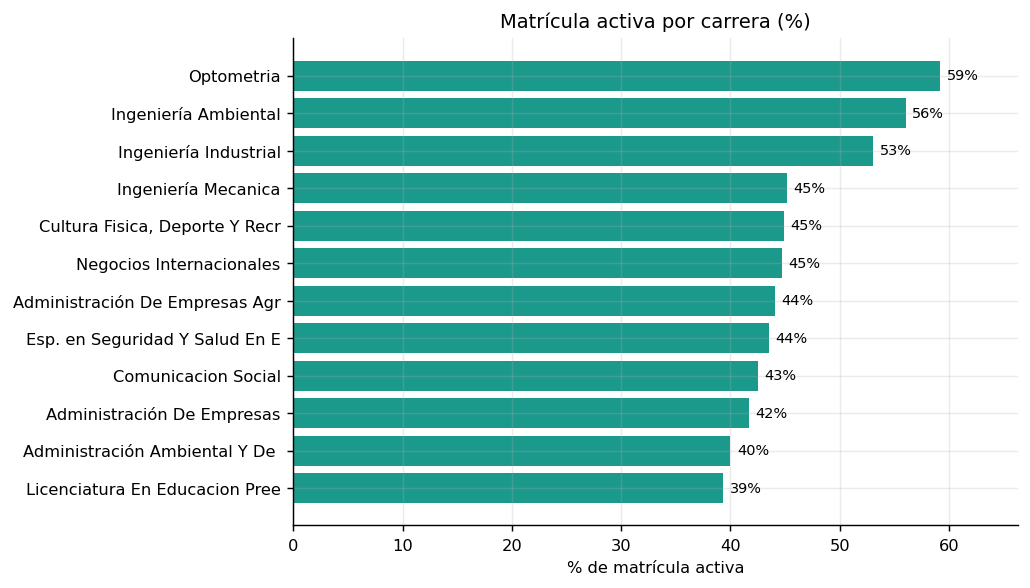
\includegraphics[width=0.74\linewidth]{figs_cruce/R3_rues_superv_carrera.png}
\caption{Porcentaje de graduados con empresa activa, por carrera (programas con un número suficiente de matriculados en el RUES).}\label{fig:ruessupcarrera}\end{figure}

Antes de sobreinterpretar esas diferencias conviene aislar un factor de confusión decisivo: la antigüedad. La Figura~\ref{fig:ruescohorte} relaciona la supervivencia con el quinquenio de la primera matrícula y el patrón es nítido: las empresas registradas hacia 2020 siguen activas en un 66,1\,\%, mientras que las de los años noventa apenas superan el 10\,\%. Es esperable ---una matrícula reciente ha tenido menos tiempo para cancelarse---, pero obliga a leer cualquier comparación de supervivencia controlando por la edad de la empresa: buena parte de las diferencias entre carreras y sedes refleja, en realidad, diferencias en la antigüedad de sus matrículas.

\begin{figure}[H]\centering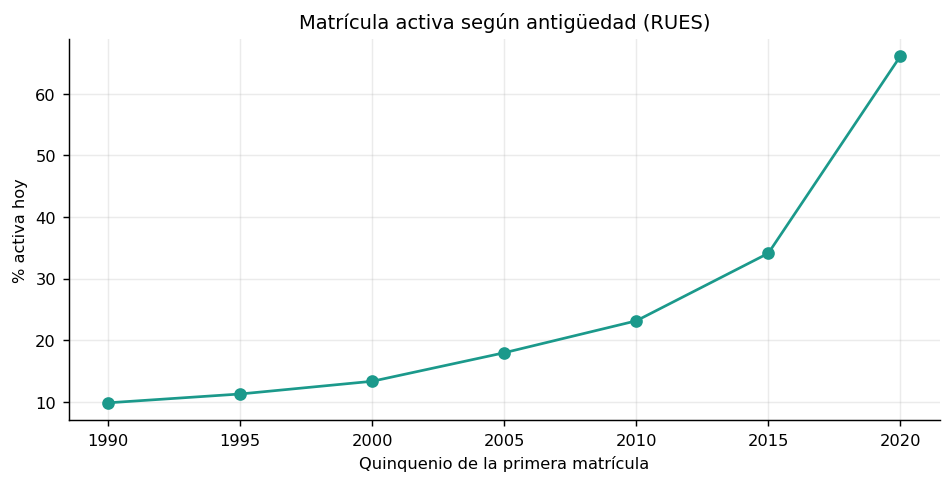
\includegraphics[width=0.74\linewidth]{figs_cruce/R4_rues_cohorte.png}
\caption{Porcentaje de empresas activas hoy según el quinquenio de la primera matrícula. La supervivencia observada depende fuertemente de la antigüedad.}\label{fig:ruescohorte}\end{figure}

\subsection{Supervivencia por sede}
Con esa cautela presente se leen las diferencias territoriales. En términos crudos, la tasa de empresa activa es del 24,1\,\% en Bogotá, del 31,6\,\% en Bucaramanga, del 40,1\,\% en Tunja, del 55,3\,\% en Villavicencio, del 33,5\,\% en Medellín y del 29,3\,\% en la VUAD. Tomado al pie de la letra, ese orden sugeriría una mayor solidez empresarial en Villavicencio; pero buena parte de la diferencia proviene de su juventud, pues, por ser una de las sedes más recientes, sus egresados registraron empresa más tarde y esas matrículas, más nuevas, han tenido menos tiempo para cancelarse.

Para separar la antigüedad del territorio conviene comparar sedes dentro de una misma cohorte de matrícula. La Figura~\ref{fig:ruessupseccoh} hace exactamente eso. Al controlar por el quinquenio de registro, la brecha se estrecha de manera notable ---en la cohorte 2015, por ejemplo, las tasas quedan en 35,7\,\% (Bucaramanga), 35,7\,\% (Tunja) y 42,9\,\% (Villavicencio), muy lejos de la diferencia cruda---, aunque Villavicencio conserva una ligera ventaja en todas las cohortes. La conclusión es matizada: la supervivencia territorial es, en su mayor parte, un artefacto de la antigüedad de las matrículas, sobre el que se monta una diferencia real pero modesta a favor de Villavicencio.

\begin{figure}[H]\centering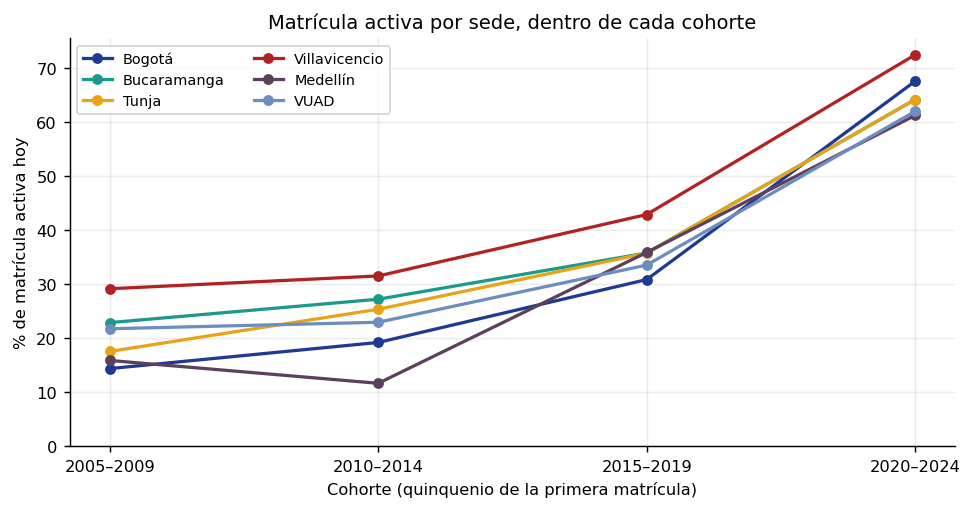
\includegraphics[width=0.78\linewidth]{figs_cruce/R5_rues_superv_seccional_cohorte.png}
\caption{Porcentaje de empresas activas por sede dentro de cada cohorte de primera matrícula. Al fijar la antigüedad, las diferencias territoriales se reducen sustancialmente.}\label{fig:ruessupseccoh}\end{figure}

\subsection{Síntesis del capítulo}
\begin{cajahallazgo}
La matrícula mercantil del egresado tomasino, tal como lo capta el RUES, es un fenómeno de persona natural volcado al comercio y los servicios de proximidad, con poco menos de un tercio de las empresas activas en la actualidad. A diferencia de la contratación pública, donde cada profesión contrata en su especialidad, en la matrícula mercantil la disciplina se diluye: salvo la salud y algunos servicios técnicos, el graduado abre negocio como comerciante antes que como profesional de su carrera. Y la supervivencia, más que un rasgo de cada programa o de cada sede, está gobernada por la antigüedad de la matrícula.
\end{cajahallazgo}

\noindent El límite de este capítulo es estructural y conviene reiterarlo. Al enlazar solo por cédula, el RUES capta la matrícula mercantil de persona natural pero deja fuera las sociedades constituidas con NIT, que son por lo común las de mayor escala y formalización. Las cifras de matrícula mercantil de este informe son, por tanto, un piso: la actividad societaria de los egresados ---probablemente la más relevante en términos económicos--- requiere un enlace adicional por nombre y representación legal que queda planteado como ampliación.
